\chapter{Baby MIND + WAGASCI}
\label{c:WAGASCI}

\section{Baby MIND}
The prototype Magnetized Iron Neutrino Detector (Baby MIND)~\cite{26babyMIND} has the principal aim to study muon charge identification efficiencies in order to get estimates for a future Neutrino Factory. A secondary aim is to compare simulations from GEANT4~\cite{Geant4} to data taken from the detector to be able to verify the properties of muon interactions at momentum ranges of 0.5 to 10 GeV/c.

The prototype is currently being built at CERN, where it will be provided with a charged particle test beam to fully understand the characteristics of the detector. Once the detector has been characterised, the plan is to integrate it into the WAGASCI experiment in Japan to improve measurements of the ratio of neutrino interaction cross-sections on water and carbon and also to place it downstream to provide improved charge identification. The main way of improving these measurements is by reducing systematic errors that arrive from the nuclear effects in water~\cite{26babyMIND}.

\subsection{Timeline}
The current timeline for the construction of Baby MIND can be seen in \FigRef{fig:timeline}.
These are the following milestones expected to be met by the Baby MIND project:
\begin{itemize}
\item Beam tests characterization at CERN in May 2017.
\item Shipment to Japan in July 2017.
\item Installation in Japan,WAGASCI pit, in September for operation in October 2017.
\end{itemize}

\begin{figure}[h!]
\centering
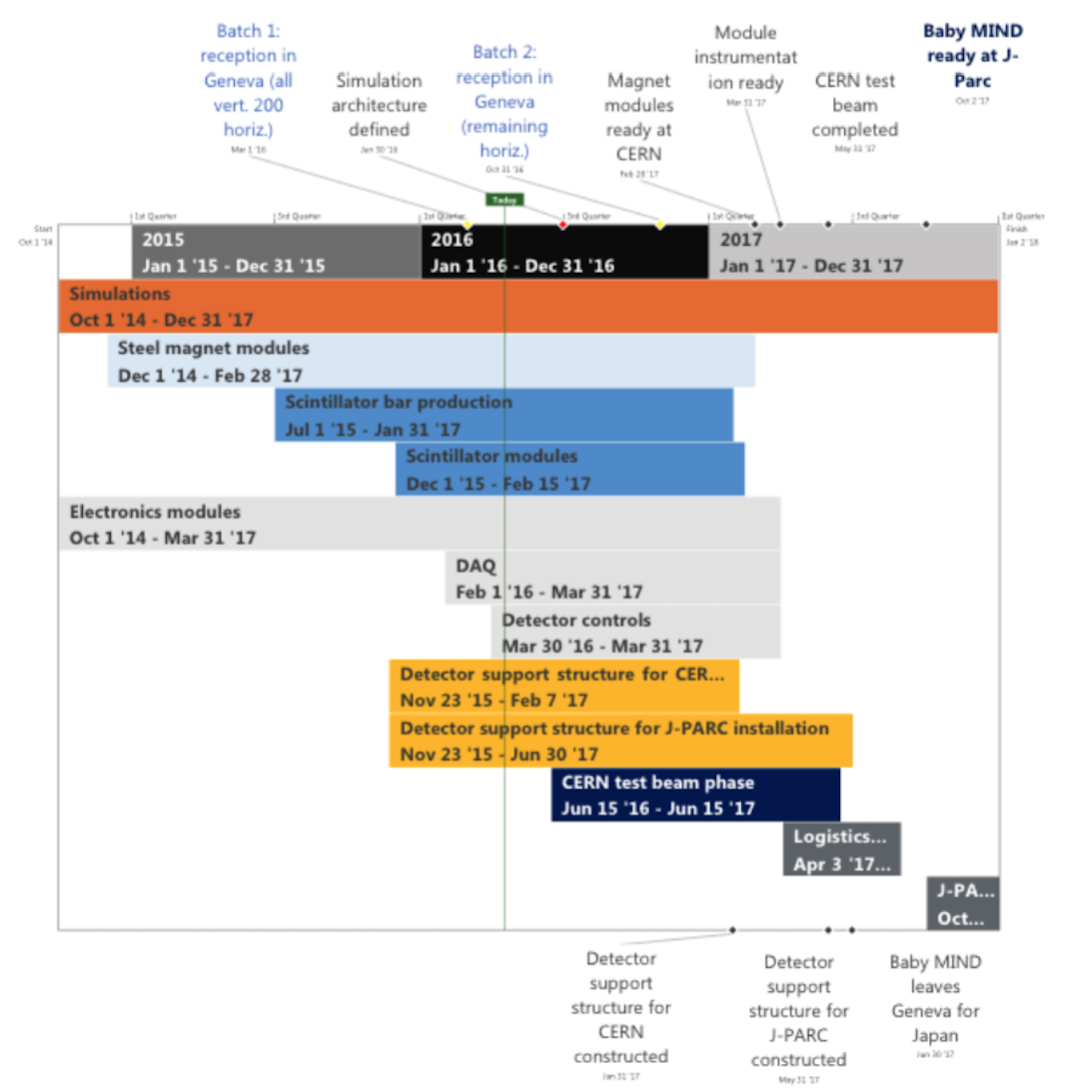
\includegraphics[width=\textwidth]{figures/timeline.png}
\caption{The current Baby MIND timeline}
\label{fig:timeline}
\end{figure}


\subsection{Collaboration}

\begin{figure}[h!]
\centering
\frame{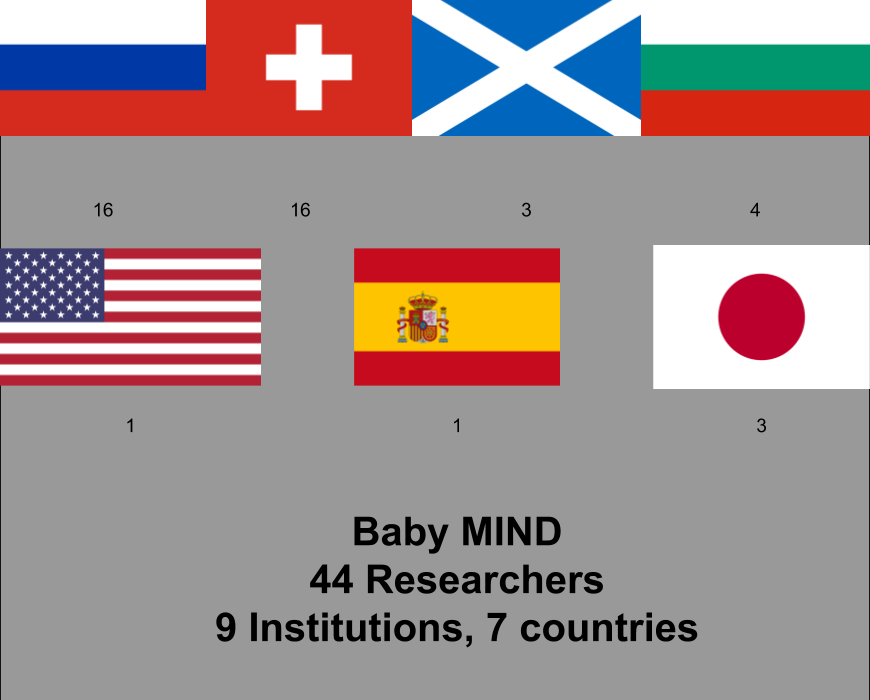
\includegraphics[width=\textwidth]{figures/Baby_MIND.png}}
\caption{The current Baby MIND collaboration}
\label{fig:collaboration}
\end{figure}

The Baby MIND collaboration is comprised of 44 scientists from nine different institutions, and is part of the CERN Neutrino Platform as experiment NP05~\cite{Fix2}.
The 3000 Multi-Pixel Photon Counters (MPPC, also known as Silicon Photomultipliers, SiPM) were provided by the University of Glasgow. Glasgow is also responsible for the simulation software.
\subsection{Layout}
As discussed in \SubSectionRef{subsec:MINDdetector}, a MIND type detector requires a magnetized volume as well as interaction medium to deflect the particle tracks and scintillating elements to detect the particle hits. A schematic overview of the detector can be seen in \FigRef{fig:design}. 
\begin{figure}[h!]
\centering
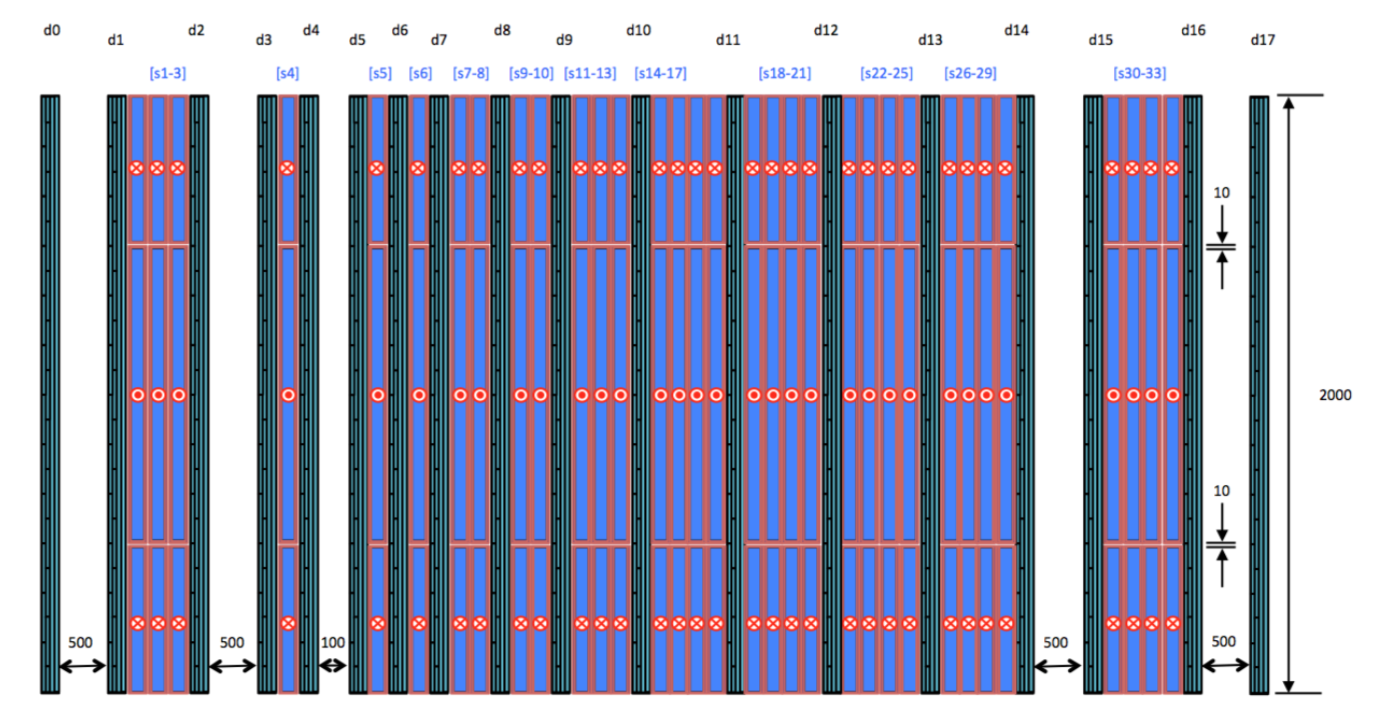
\includegraphics[width=\textwidth]{figures/design.png}
\caption{The current Baby MIND design}
\label{fig:design}
\end{figure}
The magnetised volume for the Baby MIND has been chosen as a total of 33 steel plates both to have a simple magnetic field as well as being modular and cheaper than the alternatives. An overview of the magnetic field is seen in \FigRef{fig:mField} with two open slots in order to cover the entire plate with coils with currents in opposite directions. This improves the flux return, contains the stray fields and reduces power dissipation outside of the plates compared to a single conducting coil wound on the surface of each individual plate. 

\begin{figure}[h!]
\centering
\includegraphics[width=\textwidth]{figures/MField.png}
\caption{The current Baby MIND magnetic field map}
\label{fig:mField}
\end{figure}

The scintillating elements, seen in \FigRef{fig:Vbar}, have been chosen as 18 scintillating modules consisting of four planes per module, two oriented along the horizontal direction with and two oriented in the vertical direction, each to produce good horizontal and vertical resolution of the particle interactions 

\begin{figure}[h!]
\centering
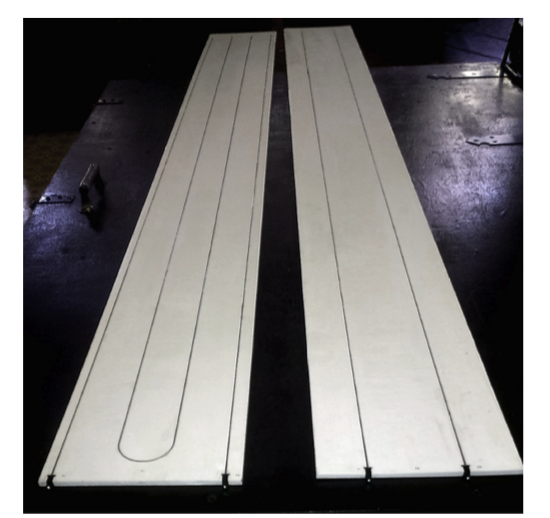
\includegraphics[width=0.5\textwidth]{figures/Vbar.png}
\caption{One of the vertical scintillator bars.}
\label{fig:Vbar}
\end{figure}
%\subsection{Motivation}
%In the white paper? LOI.

\section{WAGASCI/T59}



\subsection{Collaboration}

The current WAGASCI collaboration is given in figure~\ref{fig:collaborationW}.
\begin{figure}[h!]
\centering
\frame{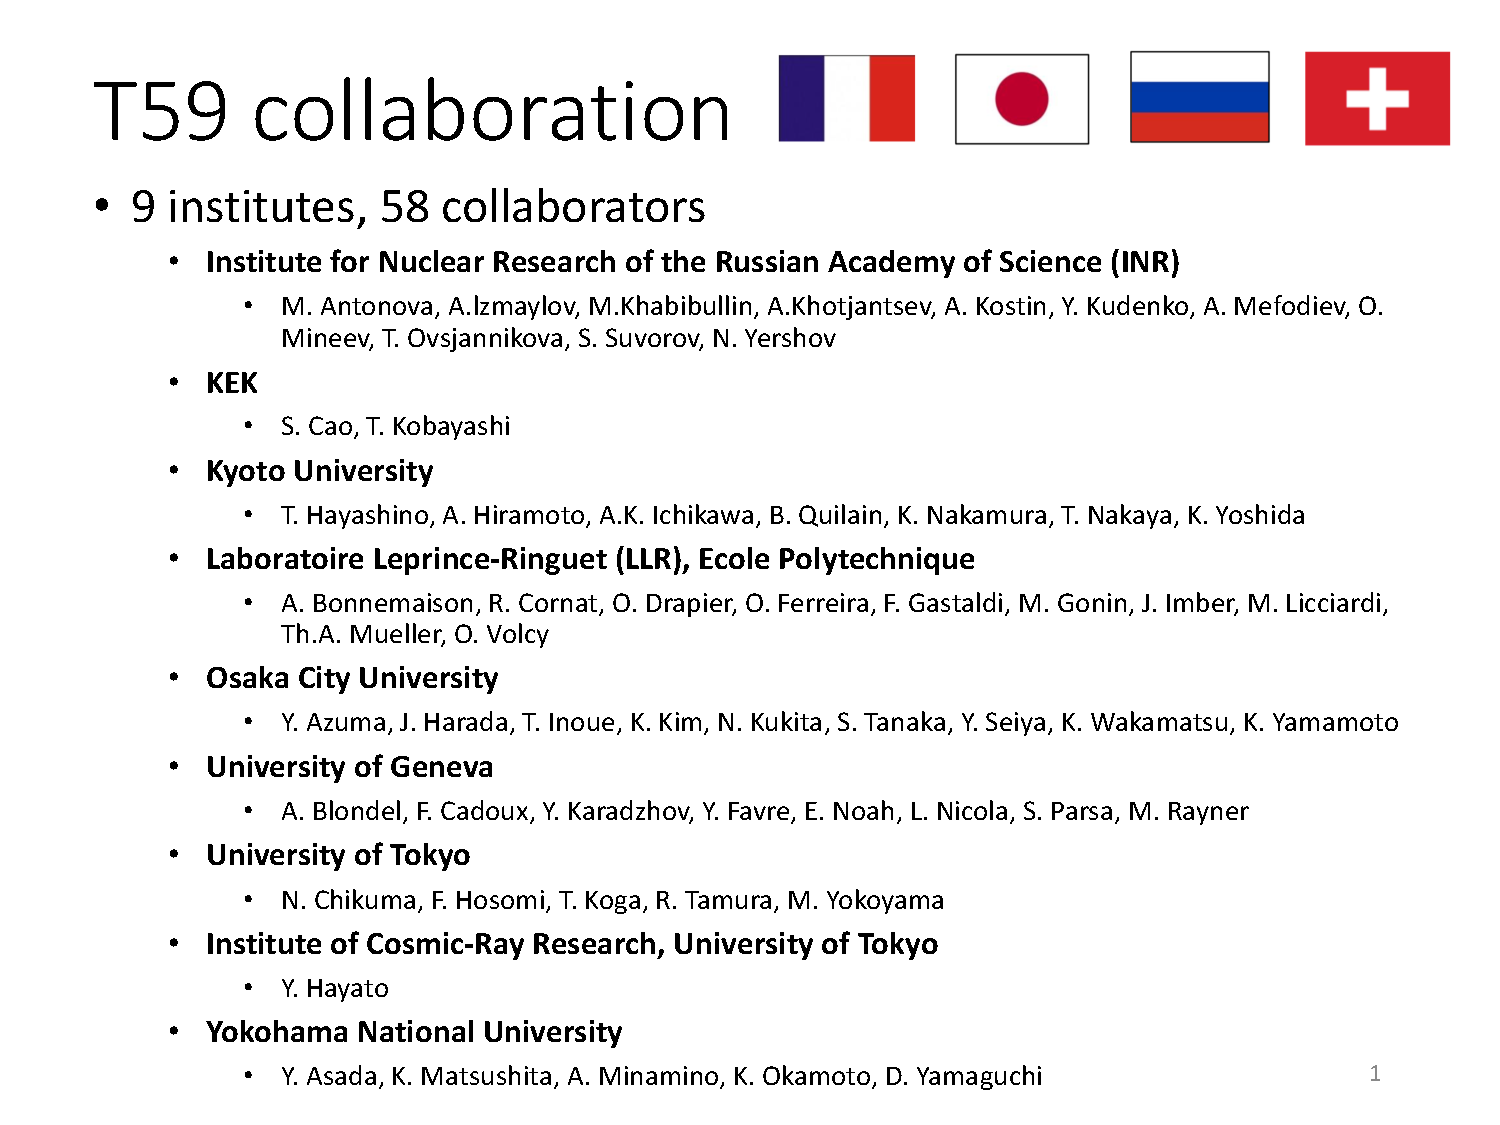
\includegraphics[width=\textwidth]{figures/T59_collaboration_18April2017.pdf}}
\caption{The current WAGASCI collaboration}
\label{fig:collaborationW}
\end{figure}

\subsection{Layout}
A new water-scintillator detector, WAGASCI (WAter- Grid-SCIintilator-Detector) seen in figure~\ref{fig:WAGASCI}, is proposed to reduce the systematic error in the T2K neutrino experiment.

\begin{figure}[h!]
\centering
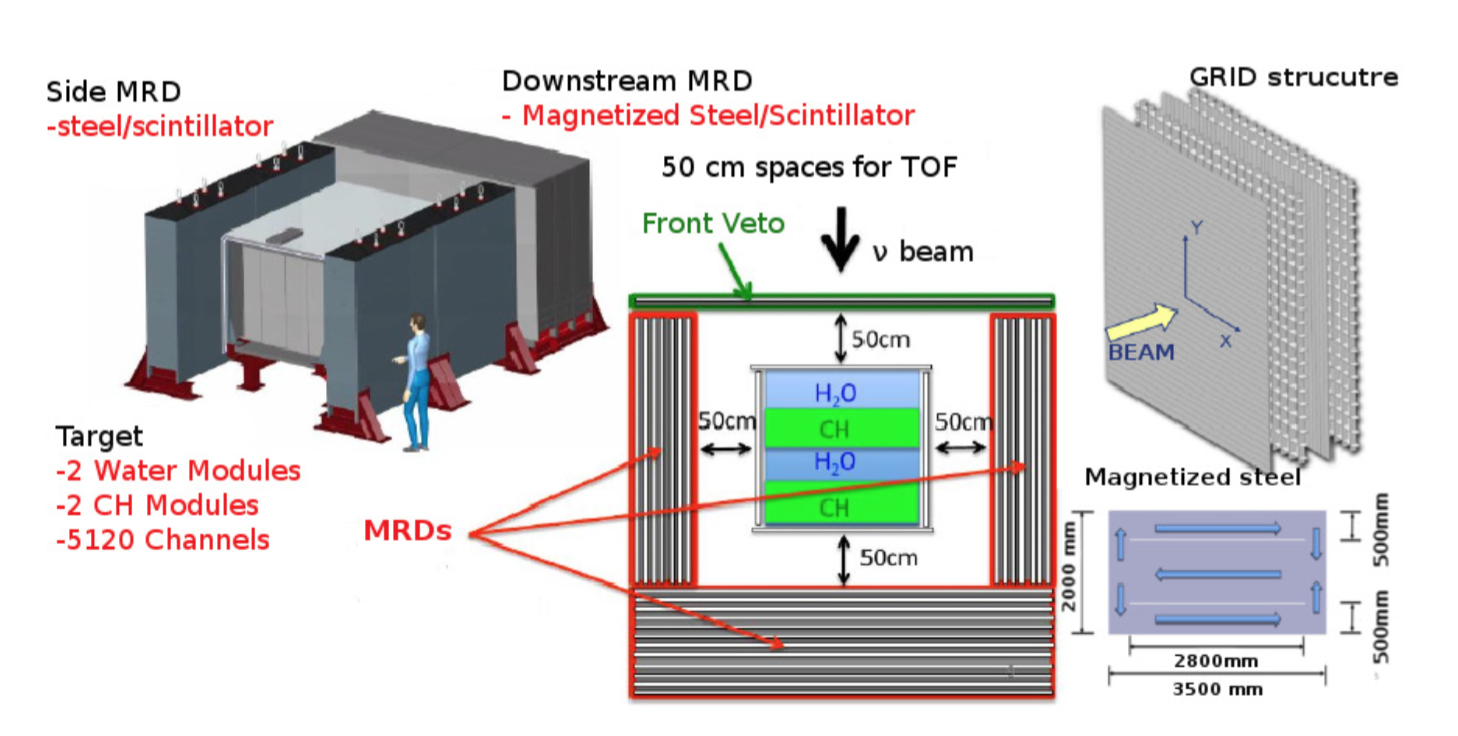
\includegraphics[width=\textwidth]{figures/WAGASCI.png}
\caption{The basic structure of the WAGASCI detector including one of the possible designs for the MIND plates.~\cite{30WAGASCI}.}
\label{fig:WAGASCI}
\end{figure}

\subsection{Motivation}
The main goals of the proposed detector are to improve the charge current cross section ratio between water and scintillator targets and to perform high-precision measurement of different charged current neutrino interaction channels.

